\documentclass[border={0.5cm 0.5cm 0.5cm 0.5cm}]{standalone}  %E,S,W,N

\usepackage{amssymb}
\usepackage{amsmath}
\usepackage{tikz}

\begin{document}
	
	%\begin{figure}
	%	\centering
	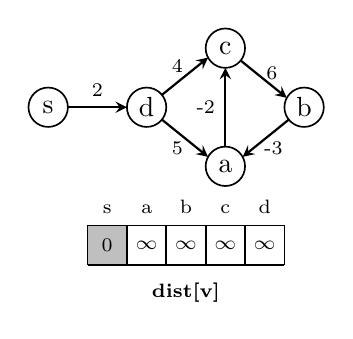
\begin{tikzpicture}
	\draw[semithick,fill=white] (0,0) circle (0.25cm);
	\node at (0,0)  {s};
	\draw[->,>=stealth,thick] (0.25,0) -- node[above] {\scriptsize 2} (1,0);
	
	\draw[->,>=stealth,thick] (1.25,0) -- node[above] {\scriptsize 4} (2.03,0.63);
	\draw[->,>=stealth,thick] (1.25,0) -- node[below] {\scriptsize 5} (2.03,-0.63);
	\draw[semithick,fill=white] (1.25,0) circle (0.25cm);
	\node at (1.25,0)  {d};
	
	\draw[->,>=stealth,thick] (2.25,0.75) -- node[right] {\scriptsize 6} (3.03,0.12);
	\draw[semithick,fill=white] (2.25,0.75) circle (0.25cm);
	\node at (2.25,0.75)  {c};
	
	\draw[->,>=stealth,thick] (2.25,-0.5) -- node[left] {\scriptsize -2} (2.25,0.5);
	\draw[semithick,fill=white] (2.25,-0.75) circle (0.25cm);
	\node at (2.25,-0.75)  {a};
	
	\draw[->,>=stealth,thick] (3.25,0) -- node[below] {\scriptsize -3} (2.47,-0.63);
	\draw[semithick,fill=white] (3.25,0) circle (0.25cm);
	\node at (3.25,0)  {b};
	
	%distance array
	\draw[step=.5cm,semithick] (0.5,-1.5) grid (3,-2);
	\filldraw[fill=lightgray,draw=black] (0.5,-1.5) rectangle (1,-2);
	%
	\draw (0.75,-1.30) node {\scriptsize s};	\draw (0.75,-1.75) node {\scriptsize 0};
	\draw (1.25,-1.30) node {\scriptsize a};	\draw (1.25,-1.75) node {\scriptsize $\infty$};
	\draw (1.75,-1.27) node {\scriptsize b};	\draw (1.75,-1.75) node {\scriptsize $\infty$};
	\draw (2.25,-1.30) node {\scriptsize c};	\draw (2.25,-1.75) node {\scriptsize $\infty$};
	\draw (2.75,-1.27) node {\scriptsize d};	\draw (2.75,-1.75) node {\scriptsize $\infty$};
	
	\node at (1.75,-2.35)  {\scriptsize \textbf{dist[v]}};
	\end{tikzpicture}
	%
	%
	\hspace{0.25cm}
	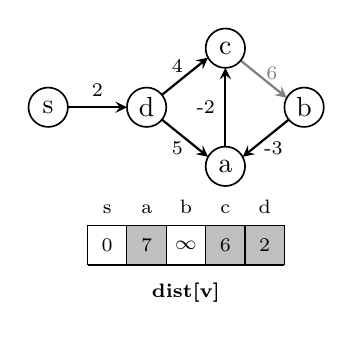
\begin{tikzpicture}
	\draw[semithick,fill=white] (0,0) circle (0.25cm);
	\node at (0,0)  {s};
	\draw[->,>=stealth,thick] (0.25,0) -- node[above] {\scriptsize 2} (1,0);
	
	\draw[->,>=stealth,thick] (1.25,0) -- node[above] {\scriptsize 4} (2.03,0.63);
	\draw[->,>=stealth,thick] (1.25,0) -- node[below] {\scriptsize 5} (2.03,-0.63);
	\draw[semithick,fill=white] (1.25,0) circle (0.25cm);
	\node at (1.25,0)  {d};
	
	\draw[->,>=stealth,thick,gray] (2.25,0.75) -- node[right] {\scriptsize 6} (3.03,0.12);
	\draw[semithick,fill=white] (2.25,0.75) circle (0.25cm);
	\node at (2.25,0.75)  {c};
	
	\draw[->,>=stealth,thick] (2.25,-0.5) -- node[left] {\scriptsize -2} (2.25,0.5);
	\draw[semithick,fill=white] (2.25,-0.75) circle (0.25cm);
	\node at (2.25,-0.75)  {a};
	
	\draw[->,>=stealth,thick] (3.25,0) -- node[below] {\scriptsize -3} (2.47,-0.63);
	\draw[semithick,fill=white] (3.25,0) circle (0.25cm);
	\node at (3.25,0)  {b};
	
	%distance array
	\draw[step=.5cm,semithick] (0.5,-1.5) grid (3,-2);
	\filldraw[fill=lightgray,draw=black] (1,-1.5) rectangle (1.5,-2);
	\filldraw[fill=lightgray,draw=black] (2,-1.5) rectangle (2.5,-2);
	\filldraw[fill=lightgray,draw=black] (2.5,-1.5) rectangle (3,-2);
	%
	\draw (0.75,-1.30) node {\scriptsize s};	\draw (0.75,-1.75) node {\scriptsize 0};
	\draw (1.25,-1.30) node {\scriptsize a};	\draw (1.25,-1.75) node {\scriptsize 7};
	\draw (1.75,-1.27) node {\scriptsize b};	\draw (1.75,-1.75) node {\scriptsize $\infty$};
	\draw (2.25,-1.30) node {\scriptsize c};	\draw (2.25,-1.75) node {\scriptsize 6};
	\draw (2.75,-1.27) node {\scriptsize d};	\draw (2.75,-1.75) node {\scriptsize 2};
	
	\node at (1.75,-2.35)  {\scriptsize \textbf{dist[v]}};
	\end{tikzpicture}
	%
	%
	\hspace{0.25cm}
	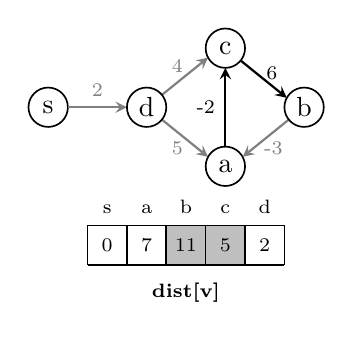
\begin{tikzpicture}
	\draw[semithick,fill=white] (0,0) circle (0.25cm);
	\node at (0,0)  {s};
	\draw[->,>=stealth,thick,gray] (0.25,0) -- node[above] {\scriptsize 2} (1,0);
	
	\draw[->,>=stealth,thick,gray] (1.25,0) -- node[above] {\scriptsize 4} (2.03,0.63);
	\draw[->,>=stealth,thick,gray] (1.25,0) -- node[below] {\scriptsize 5} (2.03,-0.63);
	\draw[semithick,fill=white] (1.25,0) circle (0.25cm);
	\node at (1.25,0)  {d};
	
	\draw[->,>=stealth,thick] (2.25,0.75) -- node[right] {\scriptsize 6} (3.03,0.12);
	\draw[semithick,fill=white] (2.25,0.75) circle (0.25cm);
	\node at (2.25,0.75)  {c};
	
	\draw[->,>=stealth,thick] (2.25,-0.5) -- node[left] {\scriptsize -2} (2.25,0.5);
	\draw[semithick,fill=white] (2.25,-0.75) circle (0.25cm);
	\node at (2.25,-0.75)  {a};
	
	\draw[->,>=stealth,thick,gray] (3.25,0) -- node[below] {\scriptsize -3} (2.47,-0.63);
	\draw[semithick,fill=white] (3.25,0) circle (0.25cm);
	\node at (3.25,0)  {b};
	
	%distance array
	\draw[step=.5cm,semithick] (0.5,-1.5) grid (3,-2);
	\filldraw[fill=lightgray,draw=black] (1.5,-1.5) rectangle (2,-2);
	\filldraw[fill=lightgray,draw=black] (2,-1.5) rectangle (2.5,-2);
	%
	\draw (0.75,-1.30) node {\scriptsize s};	\draw (0.75,-1.75) node {\scriptsize 0};
	\draw (1.25,-1.30) node {\scriptsize a};	\draw (1.25,-1.75) node {\scriptsize 7};
	\draw (1.75,-1.27) node {\scriptsize b};	\draw (1.75,-1.75) node {\scriptsize 11};
	\draw (2.25,-1.30) node {\scriptsize c};	\draw (2.25,-1.75) node {\scriptsize 5};
	\draw (2.75,-1.27) node {\scriptsize d};	\draw (2.75,-1.75) node {\scriptsize 2};
	
	\node at (1.75,-2.35)  {\scriptsize \textbf{dist[v]}};
	\end{tikzpicture}
	%	\caption{...}
	%\end{figure}
	
\end{document}